Das sogenannte Kepler-Teleskop verwendet zwei Sammellinsen mit verschiedenen
Brennweiten wie in Abbildung~\ref{10000059:fig} dargestellt.

\begin{figure}[h]
\centering
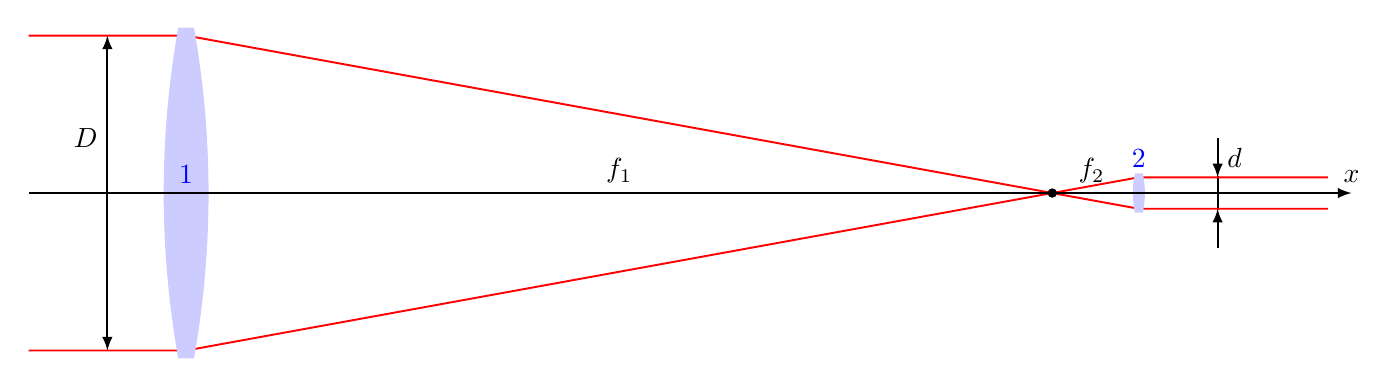
\begin{tikzpicture}[>=latex]
\def\okular{12.1}
\draw[<->,line width=0.7pt] (-1,2)--(-1,-2);
\node at (-1,0.7) [left] {$D$};
\draw[line width=0.7pt] (13.1,0.22)--(13.1,-0.22);
\draw[->,line width=0.7pt] (13.1,0.7)--(13.1,0.2);
\draw[->,line width=0.7pt] (13.1,-0.7)--(13.1,-0.2);
\node at (13.1,0.2) [above right] {$d$};
\draw[color=red,line width=0.7pt]
	(-2,2)--(0,2)--(11,0)--({\okular},-0.2)--(14.5,-0.2);
\draw[color=red,line width=0.7pt]
	(-2,-2)--(0,-2)--(11,0)--({\okular},0.2)--(14.5,0.2);
\def\rone{12.0}
\pgfmathparse{asin(2.1/\rone)}
\xdef\winkel{\pgfmathresult}
%\pgfmathparse{\rone - sqrt(\rone*\rone-2.1*2.1)+0.0}
%\xdef\done{\pgfmathresult}
\def\done{0.1}
\fill[color=blue!20]
	({-\done},{2.1}) arc ({180-\winkel}:{180+\winkel}:\rone)
	--
	({\done},{-2.1}) arc ({360-\winkel}:{360+\winkel}:\rone)
	--cycle;

\def\rtwo{1.2}
\pgfmathparse{asin(0.25/\rtwo)}
\xdef\winkel{\pgfmathresult}
\def\dtwo{0.05}
\fill[color=blue!20]
	({\okular-\dtwo},{0.25}) arc ({180-\winkel}:{180+\winkel}:\rtwo)
	--
	({\okular+\dtwo},{-0.25}) arc ({360-\winkel}:{360+\winkel}:\rtwo)
	--cycle;

\node[color=blue] at (0,0) [above] {$1$};
\node[color=blue] at ({\okular},0.2) [above] {$2$};

\draw[->,line width=0.7pt] (-2,0)--(14.8,0) coordinate[label={$x$}];
\fill (11,0) circle[radius=0.06];
\node at (5.5,0) [above] {$f_1$};
\node at (11.5,0) [above] {$f_2$};
\end{tikzpicture}
\caption{Strahlengang in einem einfachen Kepler-Teleskop
\label{10000059:fig}}
\end{figure}
Beide Linsen bestehen aus dem gleichen Material mit Brechungsindex $n=1.5$.
Die Linsen sind zudem symmetrisch (beide Flächen haben den gleichen 
Krümmungsradius). 
Der Krümmungsradius der grossen Linse ist $r_1=1000$, der der kleinen ist
$r_2=100$.
Die grosse Linse hat Dicke $d_1=10$, die kleine $d_2=6$.

\begin{teilaufgaben}
\item
Berechnen Sie die Brennweite der beiden Linsen.
\item
In welchem Abstand müssen die Linsen montiert werden, damit parallel
einfallende Lichtstrahlen auch wieder parallel aus dem System
austreten.
Dies nennt man dies ein {\em afokales} System.
Das Auge kann die parallelen Strahlen auf die Netzhaut fokusieren,
der Benutzer sieht ein scharfes Bild.
\item
Vergleichen Sie die Summe der in a) gefundenen Brennweiten mit dem
in b) gefundenen Abstand der Linsen.
\item
Ein Strahlenbündel mit Durchmesser $D$ wird beim Durchgang durch das
optische System zu einem Strahlenbündel mit Durchmesser $d$.
$d$ heisst die {\em Austrittspupille} des Systems mit Öffnung $D$.
Wenn $d$ grösser ist als die Pupille des Beobachters, kann das Auge des
Beobachters nicht alles Licht nutzen, welches das optische System liefern
kann.
\item
Mit welchem Winkel zur optischen Achse tritt ein Lichtstrahl aus,
der im Winkel $\alpha$ zur optischen Achse auf der ersten Linse
auftrifft?
Die {\em Vergrösserung} des optischen Systems ist das Verhältnis der
beiden Winkel.
\item
Vergleichen Sie die in e) gefundene Vergrösserung des Teleskops
mit dem Verhältnis der in a) gefundenen Brennweiten.
\end{teilaufgaben}

\thema{Matrixoptik}

\begin{loesung}
Die einzige Unbekannte ist $l$, der Abstand zwischen den Linsen.
Die Brechung in der Linse $i$ wird durch die Transfermatrizen
\[
B(1,n,r_i)
=
\begin{pmatrix}
1 & 0 \\
\frac1{r_i}(\frac{1}{n}-1) & \frac1{n}
\end{pmatrix}
\qquad\text{und}\qquad
B(n,1,-r_i)
=
\begin{pmatrix}
1&0\\
-\frac1{r_i}(n-1) & n
\end{pmatrix}
\]
beschrieben.

Die beiden Flächen einer Linse befinden sich im Abstand $d_i$, die
Entwicklung des Lichtstrahls zwischen den Linsen wird daher beschrieben
durch die Matrizen
\[
T_{d_i} = \begin{pmatrix} 1&d_i\\0&1\end{pmatrix}.
\]
Die Transfermatrix $T_i$ der Linse $i$ ist daher das Matrizenprodukt
\begin{equation}
T_i
=
B(n,1,-r_i)
T_{d_i}
B(1,n,r_i).
\label{10000059:linse}
\end{equation}
Diese Matrizen sind in allgemeiner Form etwas unhandlich, wir ersetzen
daher die bekannten Zahlenwerte für $r_i$, $d_i$ und $n$ und erhalten
mit Hilfe eines Computer-Algebra-Systems:
\begin{equation}
T_1
=
\begin{pmatrix}
  0.99666\overline{6}& 6.66666\overline{6}  \\
- 0.000998333\overline{3} & 0.99666\overline{6}
\end{pmatrix}
\qquad\text{und}\qquad
T_2
=
\begin{pmatrix}
 0.98 & 4.0 \\
-0.0099 & 0.98
\end{pmatrix}.
\label{10000059:linsen}
\end{equation}

Bezeichnen wir den Abstand der Linsen mit $l$.
Die Entwicklung der Lichtstrahlen zwischen den beiden Linsen wird
durch $T_l$ beschrieben.
Die Transfermatrix des Gesamtsystems ist daher
\begin{align*}
T
&=
T_2 T_l T_1.
\end{align*}
Die Radien $r_i$, die Dicke $d_i$ der Linsen und der Brechungsindex $n$
sind bekannt, aber der Abstand der Linsen $l$ ist nicht bekannt.
Einsetzen der numerischen Werte liefert 
\begin{equation}
T
=
\begin{pmatrix}
0.97274 - 0.0009783\overline{6}\cdot  l      & 0.9767\overline{3}\cdot  l + 10.52 \\
0.0000098835\cdot  l - 0.0108453\overline{6} & 0.9107\overline{3} - 0.009867\cdot l
\end{pmatrix}.
\label{10000059:gesamt}
\end{equation}


\begin{teilaufgaben}
\item 
Die Brennweite $f_i$ der Linse $i$ ist die Entfernung des Punktes auf
der optische Achse, in den parallel einfallende Strahlen konzentriert werden.
Diese Bedingung kann ausgedrückt werden als
\begin{align*}
T_{f_i} T_i\begin{pmatrix}1\\0\end{pmatrix} &= \begin{pmatrix} 0\\?\end{pmatrix}.
\end{align*}
Setzen wir die Matrizen $T_i$ aus \eqref{10000059:linsen} ein, erhalten wir
die Bedingungen
\begin{align*}
0.99\overline{6} - 0.000998\overline{3}\cdot f_1 &= 0
&
0.98 - 0.0099\cdot f_2 &= 0
\\
f_1 &= 998.33
&
f_2 &= 98.990.
\end{align*}
\item
Der Abstand $l$ muss so bestimmt werden, dass ein eintretender horizontaler
Strahl wieder als horizontaler Strahl austritt.
Horizontale Strahlen werden durch Vektoren beschrieben, die $0$ als
zweite Komponente haben.
Diese Bedingung kann also formuliert werden also die Gleichung
\[
T\begin{pmatrix}1\\0\end{pmatrix} = Te_1 = \begin{pmatrix}?\\0\end{pmatrix}.
\]
Die Bedingung an die erste Komponente des Produktes $Te_1$ ist für die
Matrix $T$ aus \eqref{10000059:gesamt}
\begin{align*}
0.0000098835\cdot l - 0.0108453\overline{6} &= 0
\\
l&=1097.3.
\end{align*}
\item
Die Summe der Brennweiten ist $f_1+f_2 = 1097.3 = l$.
Ein Kepler-Teleskop erzeugt also ein scharfes Bild für den Beobachter,
wenn die Linsen so montiert werden, dass sie einen gemeinsamen
Brennpunkt haben.
\item
Für diese Situation gilt die Gleichung
\[
T\begin{pmatrix}D\\0\end{pmatrix}=\begin{pmatrix}d\\0\end{pmatrix}
\qquad\Rightarrow\qquad
d = -0.10084\cdot D,
\]
das negative Vorzeichen bedeutet, dass die Strahlen sich kreuzen.
\item
Ein Strahl, der im Winkel $\alpha$ auf das Zentrum der Frontlinse trifft,
wird durch den Vektor
\[
\begin{pmatrix}0\\\alpha \end{pmatrix}
\]
beschrieben.
Das optische System macht daraus den Strahl, der durch
\[
T\begin{pmatrix}0\\\alpha\end{pmatrix}
=
\begin{pmatrix}
\phantom{-}
1082.31\cdot \alpha 
\\
-9.91653\cdot \alpha
\end{pmatrix}.
\]
Daraus liest man ab, dass der Winkel um den Faktor $9.92$ vergrössert
wird, das Kepler-Teleskop hat also $9.92$-fache Vergrösserung.
\item
Das Verhältnis der Brennweiten ist
\[
\frac{f_1}{f_2}
=
\frac{998.33}{98.990}
=
10.085.
\]
Dies ist ungefähr gleich gross wie die in e) berechnete Vergrösserung.
Der Unterschied rührt daher, dass wir die Brennweite von der Oberfläche
der Linse gemessen haben, nicht vom sogenannten Hauptpunkt
(principal point).
\qedhere
\end{teilaufgaben}
\end{loesung}

\begin{diskussion}
In der geometrischen Optik lernt man die Linsengleichung, mit der
sich die in dieser Aufgabe gefundenen Beziehungen für dünne Linsen
auch einfacher finden lassen.
\end{diskussion}
